\textbf{\large Результаты}

\begin{enumerate}
\item Замеры времени работы ядер с различными конфигурациями (время указано в микросекундах).

\begin{tabular}{|c|c|c|c|c|c|}\hline
\diaghead{\theadfont Diag ColumnmnHead II}%
{Конфи-\\гурации ядра}{Размер изо-\\ бражений}&
\thead{16x16}&\thead{256x256}&\thead{1280x720}&\thead{1920x1080}&\thead{3840x2160}\\
\hline
1, 32 & 453 & 158961 & 2199846 & 4599219 & 18851152\\
\hline
32, 32 & 68 & 5055 & 88657 & 168064 & 630839\\
\hline
32, 256 & 76 & 1426 & 25151 & 52567 & 217755\\
\hline
256, 256 & 75 & 1067 & 18587 & 38842 & 156823\\
\hline
1024, 1024 & 75 & 1146 & 18504 & 38516 & 160448\\
\hline
\end{tabular}

\item Сравнение с CPU

\begin{tabular}{|c|c|c|c|c|c|}\hline
Размер входных данных &
\thead{16x16}&\thead{256x256}&\thead{1280x720}&\thead{1920x1080}&\thead{3840x2160}\\
\hline
GPU(256, 256) & 75 & 1067 & 18587 & 38842 & 156823\\
\hline
CPU & 381 & 134358 & 2317364 & 4917438 & 20208486\\
\hline
\end{tabular}

\item Примеры изображений

%\begin{figure}[htb]
%{
%\centering
\begin{figure}[H]
\begin{minipage}{0.47\textwidth}
  %\centering
  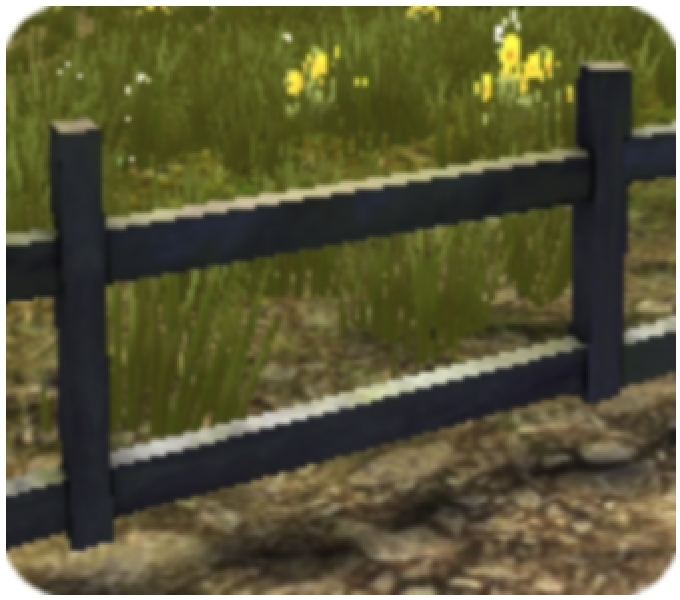
\includegraphics[width=1.0\linewidth]{src/test1.png}
  \captionof{figure}{До Махаланобиса}
  %\label{fig:test1}
\end{minipage}%
\begin{minipage}{0.47\textwidth}
  %\centering
  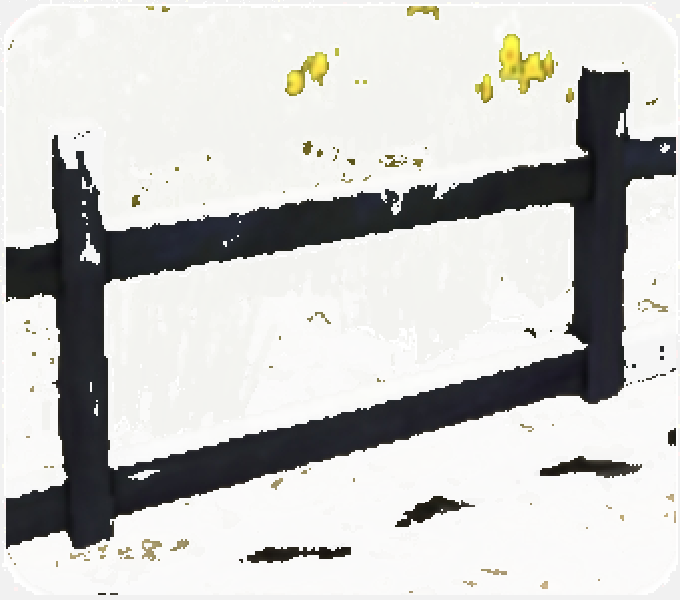
\includegraphics[width=1.0\linewidth]{src/ans1.png}
  \captionof{figure}{После Махаланобиса}
  %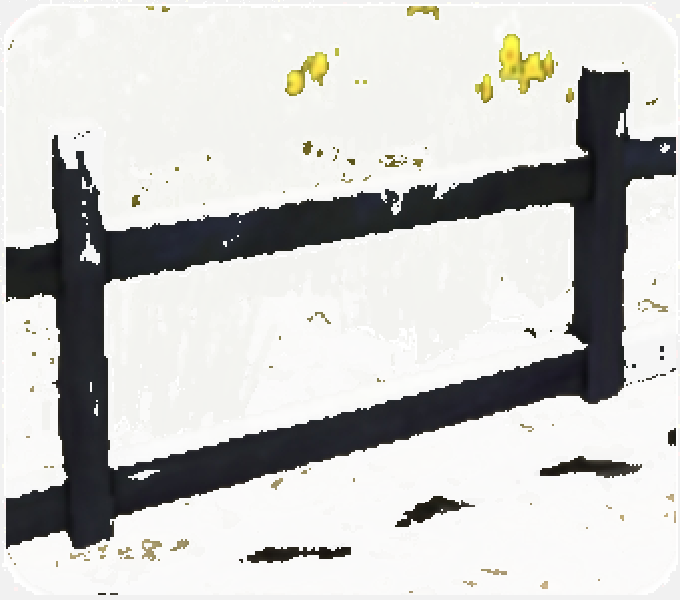
\includegraphics[width=.4\linewidth]{src/ans1.png}
  %\captionof{figure}{Another figure}
  %\label{fig:test2}
\end{minipage}
\end{figure}
%}
%\end{figure}

\begin{figure}[H]
\begin{minipage}{0.47\textwidth}
  %\centering
  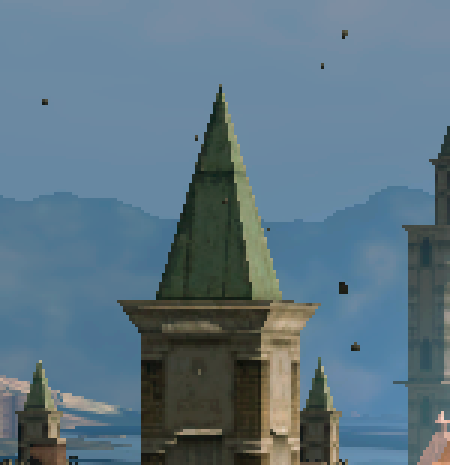
\includegraphics[width=0.95\linewidth]{src/test3.png}
  \captionof{figure}{До Махаланобиса}
  %\label{fig:test1}
\end{minipage}%
\begin{minipage}{0.47\textwidth}
  %\centering
  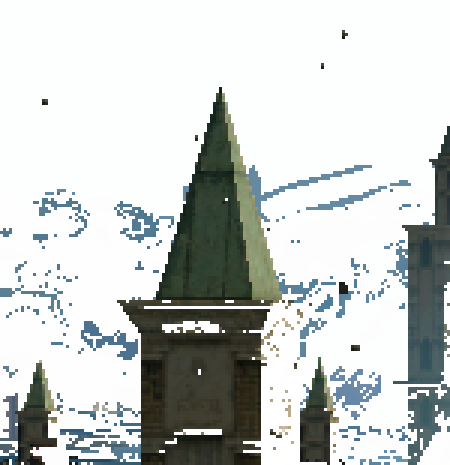
\includegraphics[width=0.95\linewidth]{src/ans3.png}
  \captionof{figure}{После Махаланобиса}
  %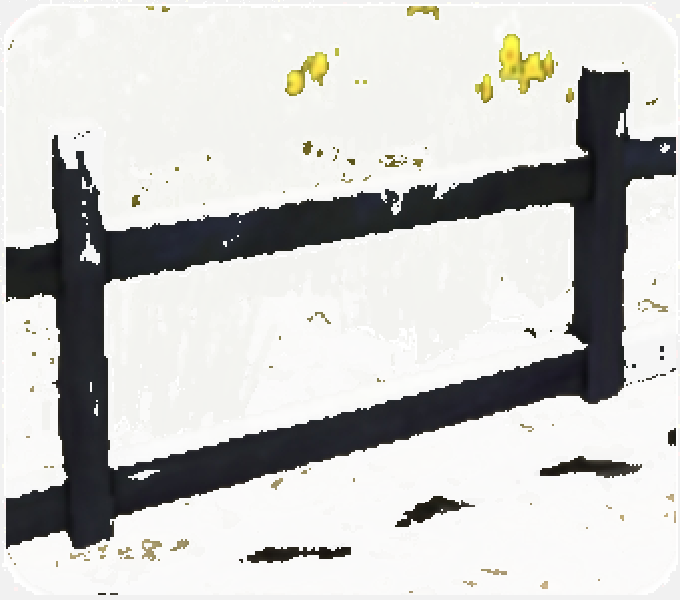
\includegraphics[width=.4\linewidth]{src/ans1.png}
  %\captionof{figure}{Another figure}
  %\label{fig:test2}
\end{minipage}
\end{figure}

\end{enumerate}

